\section{Results}
\label{sec:results}
% =============================================================

\subsection{Persistence reference}

Table~\ref{tab:persistence} reports the persistence $\rmseday$ at each site and
horizon, which defines the denominator of $\skillday$ for all models.

\begin{table}[t]
  \centering
  \caption{Persistence test-set $\rmseday$ (W/m²). All deep-learning models
           are compared against these values.}
  \label{tab:persistence}
  \begin{tabular}{lccc}
    \toprule
    \textbf{Site} & \textbf{1h} & \textbf{3h} & \textbf{6h} \\
    \midrule
    El Paso   & 204.4 & 411.0 & 565.3 \\
    Uniandes  & 293.9 & 405.0 & 470.9 \\
    \bottomrule
  \end{tabular}
\end{table}

The 1-hour persistence error at El~Paso (204.4~W/m²) is notably lower than at
Uniandes (293.9~W/m²), reflecting El~Paso's more stable clear-sky regime where
short-horizon irradiance changes are small. At 6~hours, both sites have comparable
absolute difficulty (565.3 vs.\ 470.9~W/m²).

\subsection{Main results}

Table~\ref{tab:main} reports $\rmseday$ and $\skillday$ for all models on the
test set. Deep-learning results are mean~$\pm$~std over four seeds.

\begin{table*}[t]
  \centering
  \caption{Test-set results. $\rmseday$ in W/m². $\skillday$ relative to persistence
           (higher is better). DL models: mean~$\pm$~std over 4 seeds.
           Best $\skillday$ per site-horizon highlighted in \textbf{bold}.}
  \label{tab:main}
  \setlength{\tabcolsep}{5pt}
  \resizebox{\textwidth}{!}{%
  \begin{tabular}{llcccccc}
    \toprule
    & & \multicolumn{3}{c}{\textbf{El Paso (César)}} &
         \multicolumn{3}{c}{\textbf{Uniandes (Bogotá)}} \\
    \cmidrule(lr){3-5}\cmidrule(lr){6-8}
    \textbf{Model} & \textbf{Metric} & \textbf{1h} & \textbf{3h} & \textbf{6h}
                                     & \textbf{1h} & \textbf{3h} & \textbf{6h} \\
    \midrule
    \multirow{2}{*}{Persistence}
      & $\rmseday$ & 204.4 & 411.0 & 565.3  & 293.9 & 405.0 & 470.9 \\
      & $\skillday$ & 0.000 & 0.000 & 0.000 & 0.000 & 0.000 & 0.000 \\
    \midrule
    \multirow{2}{*}{ResNet-LSTM}
      & $\rmseday$ & $238.6 \pm 22.4$ & $238.5 \pm 42.7$ & $218.4 \pm 13.2$
                   & $246.7 \pm 4.1$ & $255.7 \pm 4.8$ & $297.9 \pm 8.8$ \\
      & $\skillday$ & $\mathbf{-0.167} \pm 0.110$ & $+0.420 \pm 0.104$ & $+0.614 \pm 0.023$
                    & $\mathbf{+0.161} \pm 0.014$ & $+0.369 \pm 0.012$ & $+0.368 \pm 0.019$ \\
    \midrule
    \multirow{2}{*}{GraphSAGE-LSTM}
      & $\rmseday$ & $244.7 \pm 8.1$ & $238.9 \pm 15.9$ & $\mathbf{206.1} \pm 7.4$
                   & $250.8 \pm 5.1$ & $252.5 \pm 1.5$ & $274.4 \pm 3.9$ \\
      & $\skillday$ & $-0.197 \pm 0.040$ & $\mathbf{+0.419} \pm 0.039$ & $\mathbf{+0.636} \pm 0.013$
                    & $+0.147 \pm 0.017$ & $\mathbf{+0.376} \pm 0.004$ & $\mathbf{+0.417} \pm 0.008$ \\
    \midrule
    \multirow{2}{*}{FlatMLP (Optuna)}
      & $\rmseday$ & --- & --- & --- & --- & --- & --- \\
      & $\skillday$ & --- & --- & --- & --- & --- & --- \\
    \bottomrule
  \end{tabular}}
  \par\smallskip
  \textit{\footnotesize FlatMLP (Optuna) results are pending completion of the
  four-seed sweep (Section~\ref{sec:discussion}, Limitations) and will be
  populated prior to submission; this row quantifies what fraction of
  deep-learning skill arises from spatial encoding versus temporal dynamics
  alone.}
\end{table*}

\begin{figure*}[t]
  \centering
  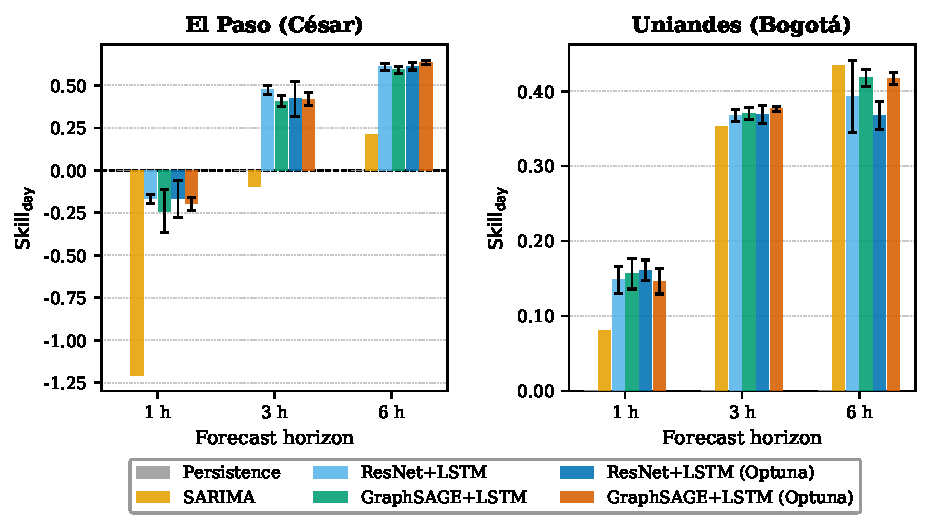
\includegraphics[width=\textwidth]{figures/fig1_skill_day}
  \caption{Daytime skill score ($\skillday$) for the deep-learning models and
           persistence at both sites across three forecast horizons. Bars show
           mean over four seeds; error bars indicate $\pm 1$ standard
           deviation. Persistence has no seed variability. GraphSAGE-LSTM
           (Optuna) achieves the highest skill among the deep-learning models
           at the 6-hour horizon at both sites (0.636 at El~Paso; 0.417 at
           Uniandes).}
  \label{fig:skill}
\end{figure*}

\begin{figure*}[t]
  \centering
  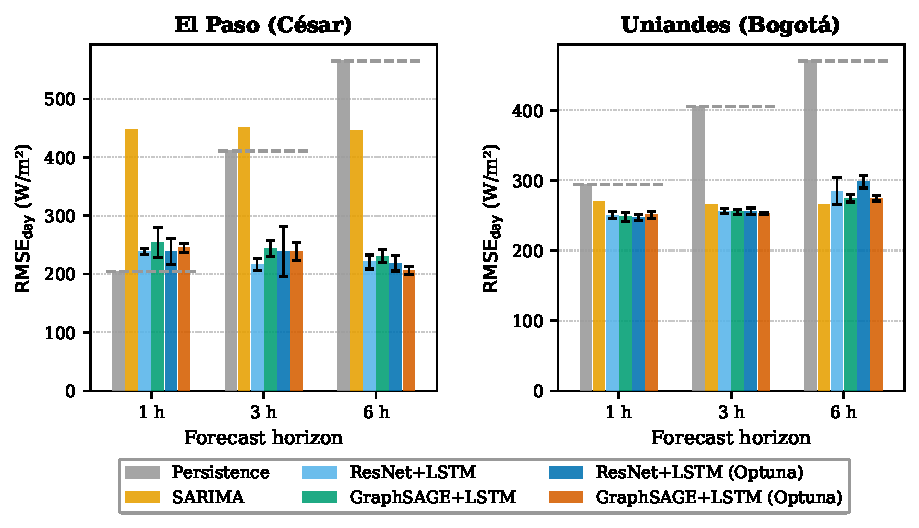
\includegraphics[width=\textwidth]{figures/fig2_rmse_day}
  \caption{Daytime RMSE ($\rmseday$, W/m²) for the deep-learning models and
           persistence. Dashed horizontal lines show the persistence reference
           for each horizon group. Both deep-learning models substantially
           reduce RMSE relative to persistence at 3h and 6h, with GraphSAGE-LSTM
           achieving the lowest RMSE at the 6-hour horizon at both sites.}
  \label{fig:rmse}
\end{figure*}

\subsection{Horizon-by-horizon analysis}

\paragraph{1-hour horizon.}
Both deep-learning models fail to beat persistence at El~Paso: ResNet-LSTM
($\skillday = -0.167 \pm 0.110$) and GraphSAGE-LSTM ($-0.197 \pm 0.040$) show
negative skill, meaning they produce higher RMSE than simply repeating the last
observation. At Uniandes the picture is more favourable: ResNet-LSTM achieves
modest positive skill ($+0.161 \pm 0.014$), narrowly ahead of GraphSAGE-LSTM
($+0.147 \pm 0.017$). The key difference between sites is the persistence
reference: El~Paso's 1-hour persistence RMSE (204.4~W/m²) is comparatively low
because irradiance changes slowly under predominantly clear-sky conditions,
leaving little room for improvement from data-driven methods. Uniandes' 1-hour
persistence RMSE (293.9~W/m²) is higher due to the frequent cloud passages,
which create more structure for the models to exploit.

\paragraph{3-hour horizon.}
Both deep-learning models outperform persistence at El~Paso by approximately
42\% ($\skillday \approx 0.42$ for both architectures, with GraphSAGE-LSTM
marginally ahead at $+0.419 \pm 0.039$). The large standard deviation for
ResNet-LSTM ($\pm 0.090$) reflects seed-to-seed variability, with some seeds
achieving near-GraphSAGE performance and others considerably below.

At Uniandes, GraphSAGE-LSTM attains the best skill at this horizon
($+0.376 \pm 0.004$), narrowly ahead of ResNet-LSTM ($+0.369 \pm 0.012$); both
are similar to each other and slightly below their El~Paso counterparts despite
the higher absolute persistence error at this site.

\paragraph{6-hour horizon.}
This is the most favourable horizon for the deep-learning models.
\textbf{GraphSAGE-LSTM achieves the best overall result}: $\rmseday = 206.1 \pm 7.4$~W/m²
and $\skillday = 0.636 \pm 0.013$ at El~Paso, reducing the persistence RMSE by
63.6\%. ResNet-LSTM is close ($0.614 \pm 0.023$) but consistently below GraphSAGE
across all seeds.

At Uniandes, GraphSAGE-LSTM again leads ($0.417 \pm 0.008$ vs.\ $0.368 \pm
0.019$ for ResNet-LSTM), with a wider margin than at El~Paso (+0.049 vs.\
+0.022 percentage points of skill). However, the \emph{absolute} skill at
Uniandes remains markedly lower than at El~Paso for both architectures ---
the gap we analyse in Section~\ref{sec:discussion}.

\begin{figure}[t]
  \centering
  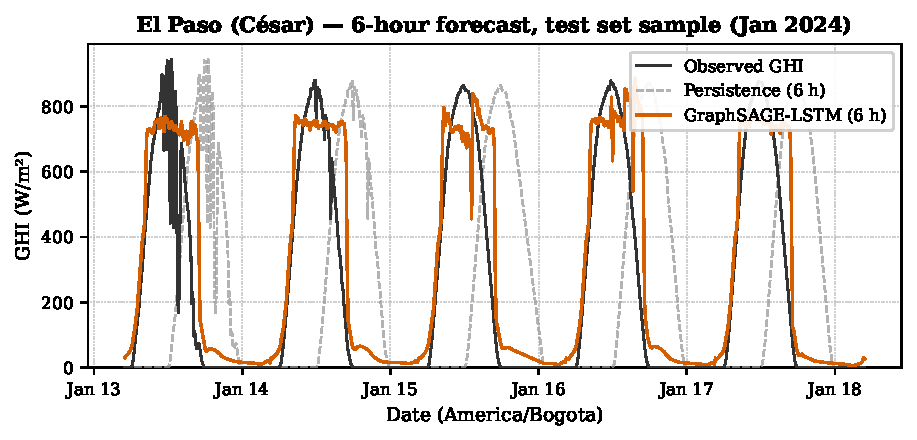
\includegraphics[width=\columnwidth]{figures/fig3_timeseries}
  \caption{Five-day excerpt of the 6-hour GHI forecast from the best model
           (GraphSAGE-LSTM Optuna, seed~42) at El~Paso in January 2024.
           Persistence (dashed) simply repeats the GHI observed 6~hours prior,
           while GraphSAGE-LSTM anticipates the diurnal rise and cloud events.
           Timestamps in local time (America/Bogotá, UTC$-5$).}
  \label{fig:ts}
\end{figure}

\subsection{Statistical robustness}

The standard deviation across seeds provides a measure of training stability.
GraphSAGE-LSTM consistently shows lower seed-to-seed variability than ResNet-LSTM
(e.g., El~Paso 6h: $\pm 0.013$ vs.\ $\pm 0.023$), suggesting that the graph
structure regularises training and reduces sensitivity to weight initialisation.
The most unstable model is ResNet-LSTM at El~Paso 3h ($\pm 0.090$), which may
reflect the interaction between the high-irradiance regime and the CNN's sensitivity
to specific initialisation-driven features.

\subsection{Conformal prediction intervals}
\label{ssec:cp_results}

Table~\ref{tab:conformal} will report the Split~CP calibration results for the
best-performing model at each site-horizon combination, evaluated at nominal
coverage levels 80\%, 90\%, and 95\%.  The conformal quantile $\hat{q}$ (W/m²)
sets the half-width of the symmetric prediction interval; daytime empirical
coverage $\hat{\text{cov}}_\text{day}$ should meet or exceed the nominal level
to satisfy the marginal coverage guarantee of Eq.~\eqref{eq:qhat}.

The backbone for El~Paso is GraphSAGE-LSTM (best overall model at 3h and 6h);
for Uniandes the best deep-learning backbone per horizon is used
(ResNet-LSTM at 1h, GraphSAGE-LSTM at 3h and 6h), consistent with
Table~\ref{tab:main}.

\begin{table*}[t]
  \centering
  \caption{Split Conformal Prediction results. $\hat{q}$: calibrated half-width (W/m²);
           $\hat{\text{cov}}_\text{day}$: empirical daytime coverage on the test set.
           Three nominal levels $1-\alpha \in \{80\%, 90\%, 95\%\}$ are reported per
           site-horizon combination. Backbone: GraphSAGE-LSTM for El~Paso;
           best-per-horizon deep-learning backbone for Uniandes (ResNet-LSTM at
           1h, GraphSAGE-LSTM at 3h and 6h).
           \textit{[Conformal calibration in progress; values to be populated prior to
           submission.]}}
  \label{tab:conformal}
  \setlength{\tabcolsep}{5pt}
  \begin{tabular}{llccccccc}
    \toprule
    & & \multicolumn{3}{c}{\textbf{El Paso}} & & \multicolumn{3}{c}{\textbf{Uniandes}} \\
    \cmidrule(lr){3-5}\cmidrule(lr){7-9}
    \textbf{Level} & \textbf{H} &
    $\hat{q}$ & $\hat{\text{cov}}_\text{day}$ & Width &&
    $\hat{q}$ & $\hat{\text{cov}}_\text{day}$ & Width \\
    \midrule
    80\% & 3h & --- & --- & --- && --- & --- & --- \\
    80\% & 6h & --- & --- & --- && --- & --- & --- \\
    \midrule
    90\% & 3h & --- & --- & --- && --- & --- & --- \\
    90\% & 6h & --- & --- & --- && --- & --- & --- \\
    \midrule
    95\% & 3h & --- & --- & --- && --- & --- & --- \\
    95\% & 6h & --- & --- & --- && --- & --- & --- \\
    \bottomrule
  \end{tabular}
\end{table*}
